\chapter{\textsc{Numération et arithmétique des ordinateurs}}
La représentation des nombres, ainsi que l'arithmétique, est très critique pour une utilisation optimale par un processeur. Historiquement on a cherché des méthodes qui minimisent le nombre d'opérations à effectuer pour réduire la taille du matériel. Bien qu'aujourd'hui ce ne soit plus si critique, c'est toujours important pour maximiser la vitesse et minimiser la consommation des processeurs.

\section{Codage binaire et hexadécimal}
Il est utile de rappeler le codage des nombres entiers positifs en base 2 et 16 avant de progresser vers les nombres négatifs et les nombres fractionnaires:

\begin{table}[!htbp]
\begin{center}
{\fontfamily{phv}\selectfont
\begin{tabular}{|c|c|c||c|c|c|}
\hline 
Entier & Binaire & Hexadécimal & Entier & Binaire & Hexadécimal\\
\hline  
0 & 0000 & 0 & 8 & 1000 & 8\\
1 & 0001 & 1 & 9 & 1001 & 9\\
2 & 0010 & 2 & 10 & 1010 & A\\
3 & 0011 & 3 & 11 & 1011 & B\\
4 & 0100 & 4 & 12 & 1100 & C\\
5 & 0101 & 5 & 13 & 1101 & D\\
6 & 0110 & 6 & 14 & 1110 & E\\
7 & 0111 & 7 & 15 & 1111 & F\\
\hline 
\end{tabular}
}
\end{center}
\caption{Codage binaire et hexadécimal des entiers positifs sur 4 bits \label{binaire hexa}}
\end{table}

%\newpage 
\section{Représentation des nombres}
Les circuits logiques, composants des processeurs, ne fonctionnent qu'en binaire. Il faut donc convertir tous les nombres usuels, pour pouvoir les utiliser. Il est aisé d'attribuer un code binaire à un nombre donné. Par exemple 000 pour le zéro et 001 pour le 1. Mais ceci devient un problème lorsqu'on ajoute le signe moins et la virgule qui ne sont pas des chiffres.

\subsection{Entiers} 
On représente les entiers positifs simplement à l'aide d'une conversion décimale-binaire directe (Table \ref{binaire hexa}).

Pour les nombres entiers négatifs nous devons faire un choix, prenons par exemple le codage avec 4 bits. Nous avons donc $2^4 = 16$ codes différents disponibles et nous devons aussi coder le zéro ce qui donne $16 - 1$ nombres disponibles. Comme c'est impaire nous aurons soit un nombre de plus du coté positif ou un nombre de plus du coté négatif. Le choix fait a été celui d'avoir un nombre négatif de plus (Table \ref{entiers négatifs}). Ce qui donne $2^{n-1}$ du côté positif pour accommoder le zéro et $2^n$ du côté négatif.

\paragraph{Complément à deux}
Il nous reste à déterminer quels codes attribuer aux nombres négatifs. En effet on peut choisir de placer les nombres négatifs à la suite des nombres positifs \textbf{ou} avant le zéro en faisant le calcul $0-1$ en binaire ou encore en décalant tous les nombres. Comparons les trois possibilités et notons bien les différences:

\begin{table}[!htbp]
\begin{center}
{\fontfamily{phv}\selectfont
\begin{tabular}{|c|c|c|c|}
\hline 
Entier & Cas 1 & Cas 2 & Cas 3\\
\hline  
\hline 
0 & 0000 & 0000 & 1000\\
\hline 
1 & 0001 & 0001 & 1001\\
\hline
7 & 0111 & 0111 & 1111\\
\hline
-1 & 1000 & 1111 & 0111\\
\hline
-2 & 1001 & 1110 & 0110\\
\hline
-8 & 1111 & 1000 & 0000\\
\hline
\end{tabular}
}
\end{center}
\caption{Trois possibilités pour coder les nombres entiers négatifs \label{entiers négatifs}}
\end{table}

On constate que le cas 1 offre une discontinuité entre -1 et 0 ce qui rend cette notation peu intéressante d'un point de vue arithmétique. Ce n'est donc pas utilisé en pratique.

Les cas 2 et 3, par contre, sont symétriques par rapport à zéro ce qui permet de faire l'opération $0-1$ sans erreur. Tous les nombres sont continus ce qui est souhaitable.

Le cas 3 à la particularité d'avoir le zéro décimal à un nombre différent du zéro binaire mais ce n'est pas un problème en soit. Ce cas est souvent utilisé pour coder l'exposant des nombres en virgule flottante et s'appelle \textbf{décalage par excès}. L'excès étant la valeur de décalage de l'échelle qui correspond au zéro décimal, e.g. 1000 = 8 (excès).

Dans le cas 2 on peut remarquer aussi que le nombre de gauche vaut "0" pour un nombre positif et "1" pour un nombre négatif, c'est pour cela qu'on l'appelle aussi bit de signe. Noter bien que si on avait choisi de coder les nombres de -7 à 8, à la place de -8 à 7, le bit de signe ne serait pas possible. Ceci est du au fait que le zéro n'a pas de signe. En pratique et en grande majorité, on préfère ce dernier et on le nomme \textbf{complément à deux}. 

Le nom \textbf{complément à deux} est une contraction de complément modulo 2. Un nombre binaire en complément à deux se calcule donc par le complément à $2^n$ du nombre non signé:
\begin{equation}
A_{comp2} = 2^n - |A|
\end{equation}
On part donc du chiffre le plus élevé et on décrémente. Exemple pour A = -1 sur 4 bits, $A_{comp2} = 2^4 - 1 = 15 = 1111$.

Le grand mérite de la notation en complément à deux est le fait qu'on peut additionner sans se préoccuper du signe alors que si on avait choisi une autre notation il aurait fallu utiliser une condition sur le signe pour en tenir compte. Pour vérifier prenons deux nombres m et r sur n bits et effectuons tous les cas de signe:

\begin{equation}
\begin{aligned}
+m \equiv m \enspace & \enspace +r \equiv r\\
-m \equiv 2^n-m \enspace & \enspace -r \equiv 2^n-r\\
(+m) + (+r) \enspace &= \enspace m + r\\
(-m) + (+r) \enspace &= \enspace 2^{n} - m + r = r-m\\
(+m) + (-r) \enspace &= \enspace m + 2^{n} - r = m-r\\
(-m) + (-r) \enspace &= \enspace 2^{n} - m + 2^{n} - r = -m-r
\end{aligned}
\end{equation}
Les $2^n$ n'affectent pas les résultats par arithmétique modulo $2^n$. On constate donc que tous les résultats sont corrects quelque soit le signe. 

\paragraph{Négation d'un nombre positif}
De la Table \ref{entiers négatifs}, on peut constater qu'il suffit d'inverser les bits du nombre positif puis d'y ajouter "1" pour obtenir la négation:

\begin{equation}
-A = \overline{A} - 1
\end{equation}

C'est une manière plus rapide de calculer le complément modulo 2. Une démonstration algébrique est donnée en annexe.
 
\paragraph{Extension d'un nombre entier}
Dans le cas ou on désire passer d'un format de n bits à m bits avec m supérieur à n, on doit remplir les cases vides m-n. Il est trivial que les cases vides d'un nombre positif doivent être des zéros, exemple, 1 sur 4 bits: 0001 et sur 8 bits: 00000001. L'extension des nombres positifs consiste donc à ajouter autant de zéros que nécessaire, mais quand est-il des nombres négatifs en complément à 2? Prenons un exemple -1 qui est 1111 sur 4 bits et si on ajoute des zéros cela donne 00001111 = 8 en complément à deux, ça ne marche pas. Pour qu'un nombre négatif reste négatif, il faut que son bit de signe soit "1", on devrait donc mettre 10001111 = -112 ce qui ne joue toujours pas. On peut trouver la réponse en faisant l'opération 0 - 1 sur 8 bits et on trouve 11111111 = -1. On constate donc que pour les nombres négatifs, il faut ajouter des "1" dans les case vides. Une démonstration algébrique vous est proposée en annexe.
 
%\newpage
\subsection{Virgule flottante}
Pour les nombre réels, on doit coder la virgule et sa position en plus du signe. Ceci complique la représentation car il faut un deuxième nombre, qui est un entier, pour représenter la position de la virgule. On choisit de préférence d'utiliser  ce nombre pour représenter un exposant plutôt qu'une position de virgule mais ça reviens au même.

\begin{equation}
X dans \, \mathbb{R} = signe \cdot m \cdot 2^{exposant}
\end{equation}

Exemple de codage avec 8 bits:
\begin{center}
{\fontfamily{phv}\selectfont
\begin{tabular}{|c|c|c|c|c|c|c|c|}
\hline
signe & m3 & m2 & m1 & m0 & e2 & e1 & e0 \\
\hline
\end{tabular}
}
\end{center}

Noter bien que l'exposant peut être positif ou négatif d'où la nécessité de choisir un format pour l'exposant comme le complément à deux ou le décalage par excès (le décalage consiste simplement à soustraire $2^{n-1}$ pour retrouver une moitié négative).

%\newpage 
\subsection{Virgule fixe}
On peut simplifier la représentation des nombre réels si la virgule est fixe, c-à-d si l'exposant ne change pas. Ceci est très utilisé dans les processeurs qui ne possèdent pas d'unité de calcul en virgule flottante.

\begin{center}
{\fontfamily{phv}\selectfont
\begin{tabular}{|c|c|c|c c|c|c|c|}
\hline
0 & 0 & 0 & 1 . & 0 & 0 & 0 & 0 \\
\hline
\end{tabular}
}
\end{center}

Dans l'exemple ci-dessus nous avons 4 bits pour le nombre entier et 4 bits pour le nombre fractionnaire. La virgule n'est pas codée en tant que tel et le nombre complet utilise 8 bits. Seul deux constantes sont nécessaires pour décrire le format en virgule fixe: la longueur de la partie entière et la longueur de la partie fractionnaire:

\lstset{style=customc}
\begin{lstlisting}
#define FIXEDPT_IBITS	4
#define FIXEDPT_FBITS	4
\end{lstlisting}

\section{Opérateurs}
Les opérations arithmétiques sont différentes pour chaque format de nombre mais elles peuvent toutes se ramener à un additionneur 1 bit qui se réalise facilement à l'aide d'un porte logique XOR et AND. 

\begin{table}[!htbp]
\begin{center}
{\fontfamily{phv}\selectfont
\begin{tabular}{|c|c|c|c|}
\hline 
A & B & A + B & Retenue\\
\hline  
\hline 
0 & 0 & 0 & 0\\
\hline 
0 & 1 & 1 & 0\\
\hline
1 & 0 & 1 & 0\\
\hline
1 & 1 & 0 & 1\\
\hline
\end{tabular}
}
\end{center}
\caption{Table de vérité de l'additionneur 1 bit \label{add 1 bit}}
\end{table}

\begin{figure}[htb]
  \centering
  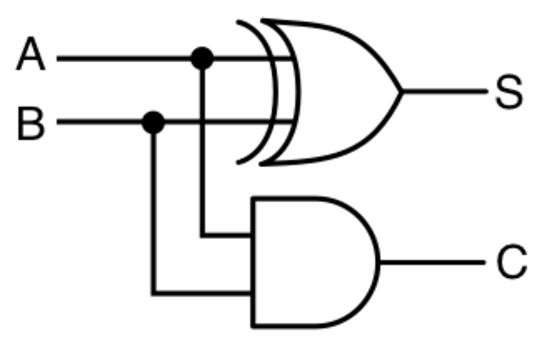
\includegraphics[width=5cm]{./Figures/arith/Half-adder.pdf}
  \rule{35em}{0.5pt}
  \caption[half_adder]{Réalisation de l'additionneur 1 bit (sans entrée de retenue)}
  \label{fig:half_adder}
\end{figure}

Le circuit complet d'un additionneur 1 bit doit encore sommer une retenue éventuelle en entrée donc en réalité il additionne 3 bits. Exactement de la même manière que lorsqu'on calcule en colonnes à la main.

\subsection{Addition}
Additionner deux nombres entiers positifs est évident mais attention aux débordements! Par exemple: 4 + 4 = 8, sur 4 bits (n=4) en complément à deux, nous n'avons pas de code pour le 8. Pour comprendre ce qu'il se passe, effectuons l'addition en binaire:

\begin{center}
{\fontfamily{phv}\selectfont
\begin{tabular}{c c c}
  & 0100 & 4 \\
+ & 0100 & 4 \\
\hline
  & 1000 & -8 \\
\end{tabular}
}
\end{center}

Selon ce calcul, nous avons donc un résultat de -8 à la place de +8. Il faut donc un mécanisme pour nous avertir quand un débordement se produit (voir chapitre 8).

Nous avons un problème similaire lors de l'addition de deux nombres entiers négatifs, par exemple: -4 + (-5) = -9. Si nous faisons le calcul en représentation en complément à deux sur 4 bits:

\begin{center}
{\fontfamily{phv}\selectfont
\begin{tabular}{c c c}
  & 1100 & -4 \\
+ & 1011 & -5 \\
\hline
  & 0111 & +7 \\
\end{tabular}
}
\end{center}

On peut constater que le débordement conduit à retourner au nombre le plus élevé de l'autre côté de la gamme. En binaire, le calcul s'effectue, débordement ou pas, et le processeur continue comme si de rien n'était. On appelle ceci, l'arithmétique modulo $2^n$. L'opération modulo, par exemple en langage C, retourne le reste de la division entière d'un nombre. Cette opération s'effectue automatiquement à l'aide d'une addition en arithmétique modulo, par exemple en représentation 4 bits non-signée: (8 + 9) modulo 16 = 1. Pour bien comprendre effectuons l'addition en binaire:
 
\begin{center}
{\fontfamily{phv}\selectfont
\begin{tabular}{c c c}
  & 1000 & 8 \\
+ & 1001 & 9 \\
\hline
  & 0001 & 1 \\
\end{tabular}
}
\end{center}

Le résultat de l'addition est bien celui du reste de la division entière par 16.

L'addition en virgule fixe reste la même que l'addition pour les entiers mais l'addition en virgule flottante est très différente car il faut ajuster l'exposant.

\subsection{Soustraction}
La soustraction peut se décomposer en un changement de signe et une addition ce qui permet de se ramener aux cas ci-dessus. 

\begin{equation}
A - B = A + (-B)
\end{equation}

De plus un seul composant matériel, l'additionneur, est nécessaire pour les deux opérations. La négation ne nécessite qu'une inversion et l'ajout de "1" qui s'effectue aussi à l'aide du même additionneur.

\subsection{Multiplication}
On peut décomposer une multiplication en sommes de produits qui se ramène d'un point de vue matériel à des additions et des décalages. Prenons un exemple 3 x 5 sur 4 bits (n=4) non signé:

\begin{center}
{\fontfamily{phv}\selectfont
\begin{tabular}{c r r}
  & 0011 & 3 \\
x & 0101 & 5 \\
\hline
& 00000011 \\
& 00000000 \\
& 00001100 \\
& 00000000 \\
\hline
& 00001111 & 15 \\
\end{tabular}
}
\end{center}

On constate donc qu'il suffit de créer quatre produits intermédiaires qui sont juste des décalages du nombre 3 lorsque le nombre multipliant est non nul. Ensuite on fait la somme des quatre nombres avec un additionneur. Noter bien que si on décale de 4 crans vers la gauche, le nombre intermédiaire à une taille de 8 bits. Les résultats sont donc sur $2n$ bits.

Le cas des nombres négatifs est différent au niveau de l'extension des nombres intermédiaires. En effet, dans notre multiplication ci-dessus nous avons introduit des zéros pour étendre un nombre. Prenons l'exemple suivant (-3) x 2 sur 4 bits signés:

\begin{center}
{\fontfamily{phv}\selectfont
\begin{tabular}{c r r}
  & 1101 & -3 \\
x & 0010 & 2 \\
\hline
& 00000000 \\
& 11111010 \\
& 00000000 \\
& 00000000 \\
\hline
& 11111010 & -6\\
\end{tabular}
}
\end{center}

Dans ce cas ci, nous devons étendre le nombre intermédiaire négatif avec des "1" pour obtenir la bonne solution. Le résultat reste -6 quelque soit le nombre de "1" devant le nombre (1010 = -6, 11111010 = -6). Le changement des bits de l'extension nécessite une condition sur le signe qui rend le calcul d'un nombre signé plus long que celui d'un nombre non-signé. Il faut donc une autre technique pour un processeur qui est indépendante du signe.

La multiplication de nombres en virgule fixe est légèrement différente car il faut décaler le résultat de multiplication de la taille de la partie fractionnaire vers la droite:

\lstset{style=customc}
\begin{lstlisting}
#define FIXEDPT_IBITS	8
#define FIXEDPT_FBITS	8

typedef int16_t fixed16_t;

/**
 * Multiplies two fixed16_t numbers
 * @param a
 * @param b
 * @return a * b
 */
inline fixed16_t fixed16_mul(fixed16_t a, fixed16_t b)
{
	return (((fixed16_t)a * (fixed16_td)b) >> FIXEDPT_FBITS);
}
\end{lstlisting}

Le but de ce décalage est de replacer la virgule au bon endroit dans le résultat car le nombre de bits de la partie fractionnaire vaut $2n$ et donc il faut le décaler de $n$ à droite.

\paragraph{Réduction de la complexité du calcul de la multiplication}
En faisant le calcul selon la méthode en colonnes trois problèmes se posent:
\begin{enumerate}
\item Le nombre de produits intermédiaires est de $n$ ce qui nécessite $n$ emplacements de mémoire sous forme de registres rapides pour effectuer le calcul à la vitesse maximum. 
\item La taille des résultats intermédiaires vaut $2n$ donc il faut des emplacements mémoire doubles.
\item Si une des opérandes est négative alors il faut calculer sans le signe puis effectuer une correction
\end{enumerate}
Le premier problème peut se résoudre en accumulant le résultat intermédiaire au fur et à mesure. Le deuxième en ne mémorisant que les n bits de poids fort. Le dernier problème en utilisant l'\textbf{algorithme de Booth} (voir annexe \ref{ch:algebra}). 

\subsection{Division}
La division entière ou Euclidienne est très simple à implémenter à l'aide de la soustraction successive du diviseur:

\lstset{style=customc}
\begin{lstlisting}
int divide(N, D) {
	Q = 0;
	while (N >= D) {
  		N = N - D;
  		Q++;
	}
	return Q;			//ou N pour le reste
}
\end{lstlisting}

La division entière peut donc s'effectuer avec un additionneur, une négation et un test. Le temps d'exécution est par contre relativement long si N>>D.

Pour le cas de la virgule fixe, il faut décaler le multiplicande vers la gauche avant division:

\lstset{style=customc}
\begin{lstlisting}
#define FIXEDPT_IBITS	8
#define FIXEDPT_FBITS	8

typedef int16_t fixed16_t;

/**
 * Divides two fixed16_t numbers
 * @param a
 * @param b
 * @return a / b
 */
inline fixed16_t fixed16_div(fixed16_t a, fixed16_t b)
{
	return (((fixed16_t)a << FIXEDPT_FBITS) / (fixed16_t)b);
}
\end{lstlisting}

Comme pour la multiplication, il existe des algorithmes plus efficaces pour faire la division entière comme celui appelé SRT.

\section{Exercices}

\paragraph{Ex 1}
Implémenter l'algorithme de Booth en C puis en assembleur.

\paragraph{Ex 2}
Écrire en C une fonction de division de deux nombres entiers en complément à 2 qui retourne le résultat en utilisant seulement des additions ou des soustractions. Attention aux signes et à la division par zéro.

\paragraph{Ex 3}
Implémenter l'algorithme SRT en C.


